\documentclass[tikz,border=1pt]{standalone}
\usetikzlibrary{shapes.geometric, arrows.meta, positioning, fit, backgrounds}
\begin{document}
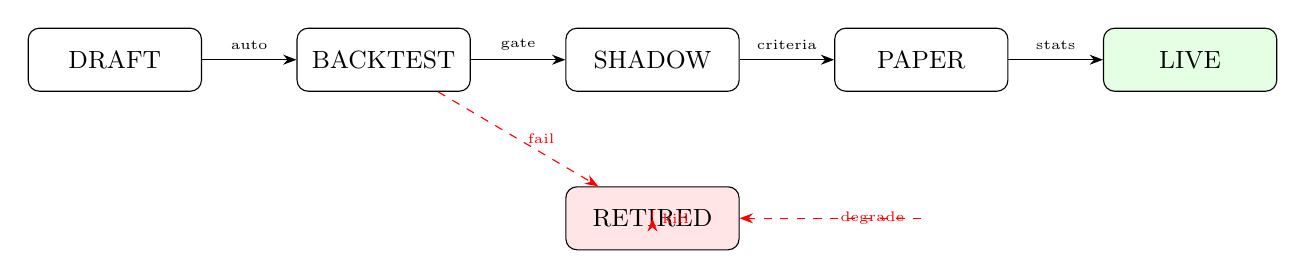
\begin{tikzpicture}[node distance=1.2cm, >={Stealth},
    stage/.style={draw, rectangle, rounded corners, minimum width=2.2cm, minimum height=0.8cm, align=center, font=\small}]
    \node[stage] (d) {DRAFT};
    \node[stage, right=of d] (b) {BACKTEST};
    \node[stage, right=of b] (s) {SHADOW};
    \node[stage, right=of s] (p) {PAPER};
    \node[stage, right=of p, fill=green!10] (l) {LIVE};
    \node[stage, below=1.2cm of s, fill=red!10] (r) {RETIRED};
    \draw[->] (d) -- node[above, font=\tiny]{auto} (b);
    \draw[->] (b) -- node[above, font=\tiny]{gate} (s);
    \draw[->] (s) -- node[above, font=\tiny]{criteria} (p);
    \draw[->] (p) -- node[above, font=\tiny]{stats} (l);
    \draw[->, red, dashed] (b) -- node[right, font=\tiny]{fail} (r);
    \draw[->, red, dashed] (s|-r) -- node[right, font=\tiny]{kill} (r);
    \draw[->, red, dashed] (p|-r) -- node[right, font=\tiny]{degrade} (r);
\end{tikzpicture}
\end{document}
